En este capítulo se presentará una revisión exhaustiva de la literatura existente relacionada con la toma de decisiones en conducción autónoma. A través de investigaciones previas relacionadas con la temática, se expondrá el estado actual y los retos que plantean los vehículos autónomos, desde investigaciones que abordan desde una perspectiva global hasta trabajos más específicos relacionados con la información adquirida por los sensores.

\section{Vehículos autónomos: actualidad y desafíos}

La seguridad en la industria del automóvil es uno de los temas que más preocupa a la sociedad actual. A pesar de los avances tecnológicos realizados en las últimas décadas, los accidentes de tráfico se siguen considerando una de las principales causas de muerte en todo el mundo, con proyección de aumentar en un futuro próximo (\cite{who2018}). El último estudio publicado por la Agencia Nacional de Seguridad Vial Americana, en inglés \gls{nhtsa}, reveló que la principal causa de los siniestros graves es el factor humano, en el cual se engloban errores como el reconocimiento, la decisión y la ejecución principalmente (\cite{nhtsa18}). 

Los vehículos autónomos proyectan un futuro más seguro y confiable para los conductores, paliando los problemas derivados de la conducción manual y descargando al conductor del procesamiento de información. El desarrollo de la conducción autónoma posee muchas ventajas que benefician a la sociedad como son la reducción de la siniestralidad, la liberación de espacios dedicados a aparcamientos, el compromiso medioambiental y la nueva gestión del tiempo dedicado a la conducción (\cite{terrones}). Para entender su campo de actuación es necesario explicar los niveles en los que se dividen y sus funciones. En 2014, la \gls{sae} estableció seis niveles de automatización, del 0 al 5, los cuales comprendían desde la conducción manual hasta la automatización total. 

En abril de 2021 se realiza la última actualización de dicha clasificación, donde se perfecciona la separación entre los niveles 3 y 4 y se extienden los primeros niveles ajustándose a los avances desarrollados (\cite{sae}). En la figura \ref{fig:2.1} se muestra un esquema proporcionado por \gls{sae} con las características de cada nivel adaptado al español.

\newpage
\begin{figure}[htb]
  \centering
  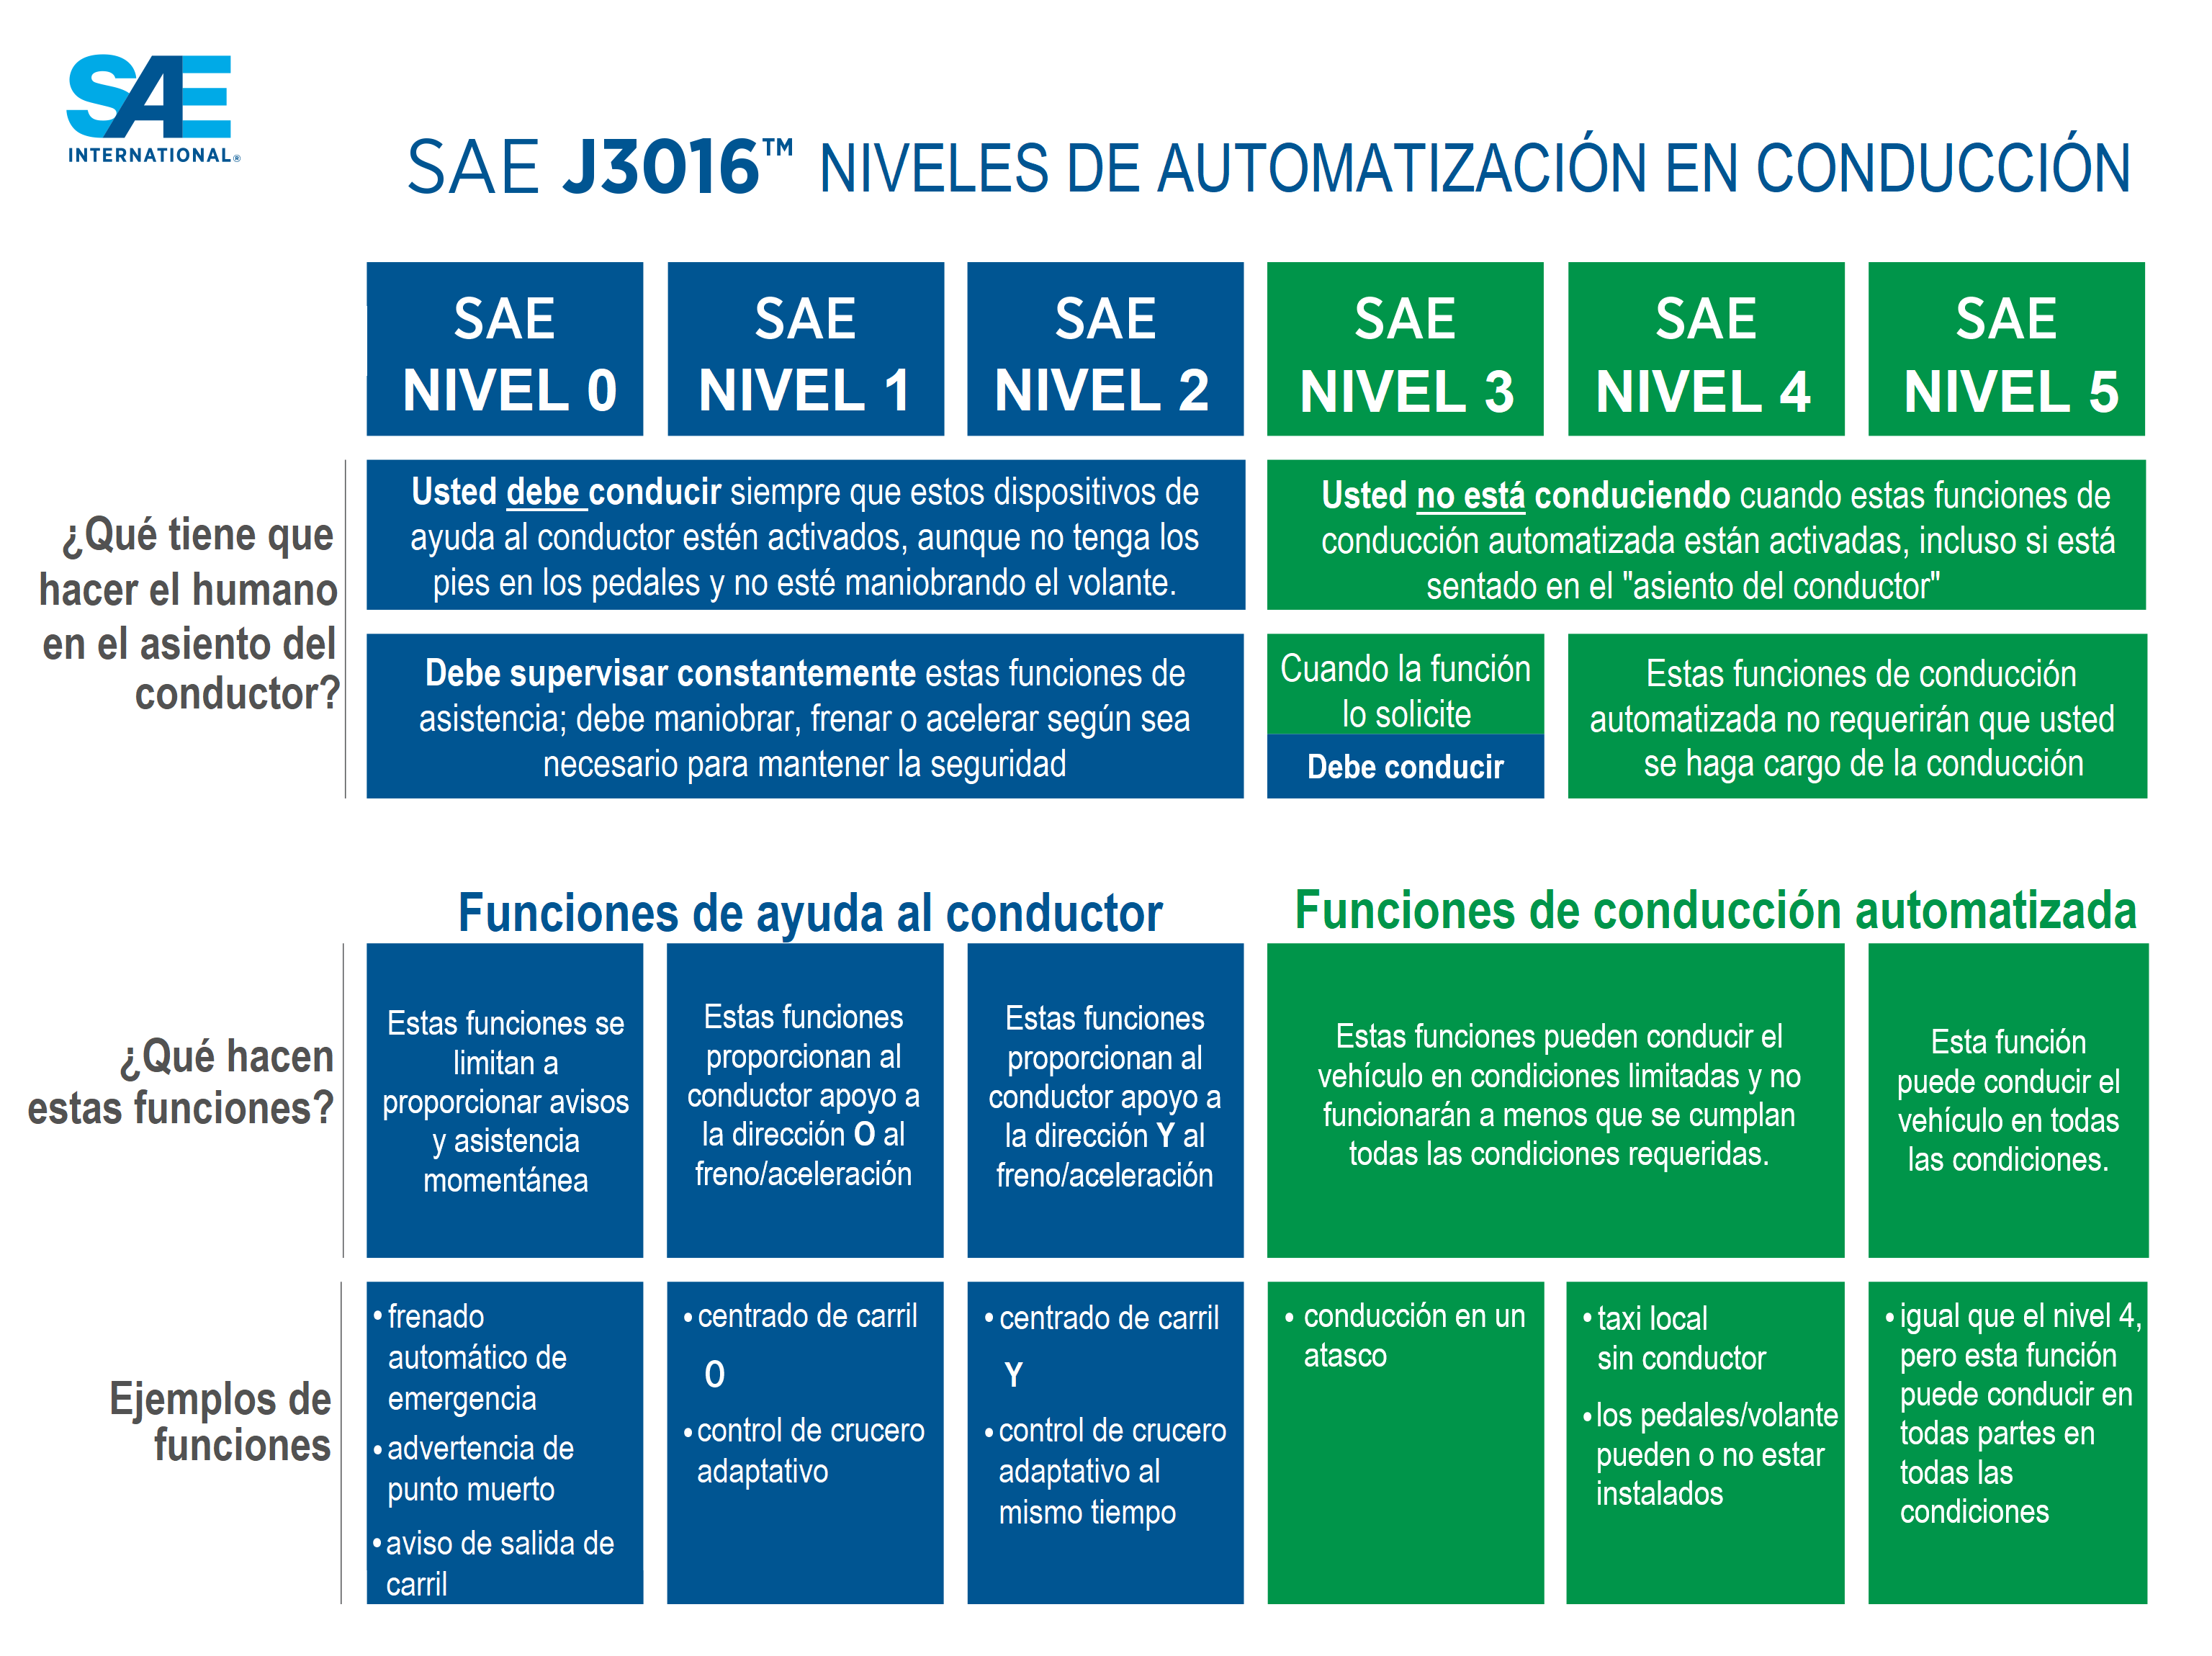
\includegraphics[width=13.5cm]{figures/2.1.png}
  \caption{\label{fig:2.1} Niveles de automatización en conducción (original en \textcite{sae}).}
\end{figure}

De igual manera, en junio de 2022 la \gls{nhtsa} publicó unos informes sobre accidentes relacionados con la conducción autónoma a lo largo de un año, gracias a los reportes proporcionados por los fabricantes de vehículos en diferentes niveles de automatización. Estos resultados aportan transparencia sobre la seguridad de dichos vehículos y proporcionan datos importantes para la investigación y para el desarrollo de políticas que mejoren la seguridad en estas tecnologías. A pesar de que dichos resultados son poco representativos, debido a la naturaleza de la muestra, permiten vislumbrar unos primeros resultados a nivel proporcional. Los informes se dividen en dos, accidentes para vehículos hasta nivel 2 equipados con sistemas avanzados de asistencia al conductor, en inglés \gls{adas} (\cite{nhtsa22a}) y accidentes para vehículos en los niveles 3-5 de automatización (\cite{nhtsa22b}). 

Los fabricantes que más datos reportaron fueron Tesla y Honda para vehículos hasta nivel 2, y Waymo y Transdev para niveles superiores de automatización. Las colisiones con otros vehículos de la vía, fueron alrededor de un 30\% para vehículos hasta nivel 2 y un 80\% para el resto de niveles, notándose los problemas actuales de integración de la conducción altamente automatizada con el tráfico mixto (Figura \ref{fig:2.2} y Figura \ref{fig:2.3}). 

\newpage
\begin{figure}[h]
  \centering
  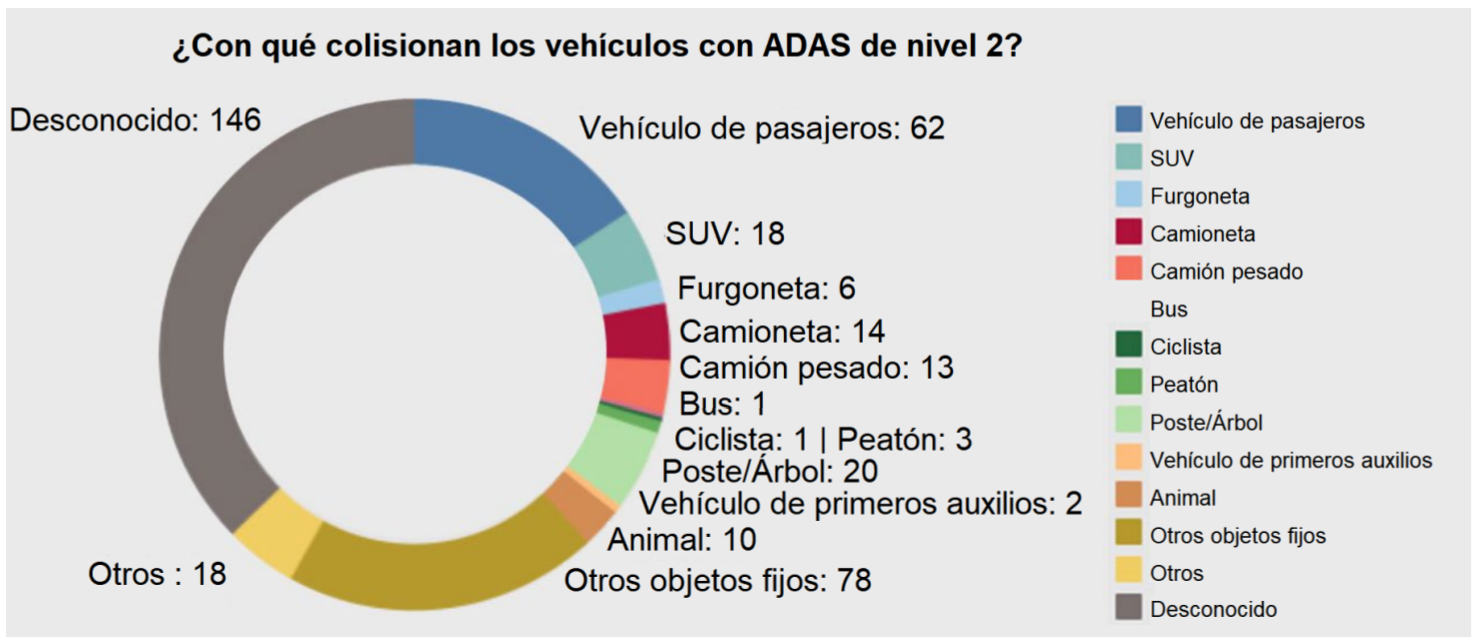
\includegraphics[width=12.5cm]{figures/2.2.png}
  \caption{\label{fig:2.2} Colisiones de vehículos autónomos con \gls{adas} de nivel 2 (original en \textcite{nhtsa22a}).}
\end{figure}

\begin{figure}[h]
  \centering
  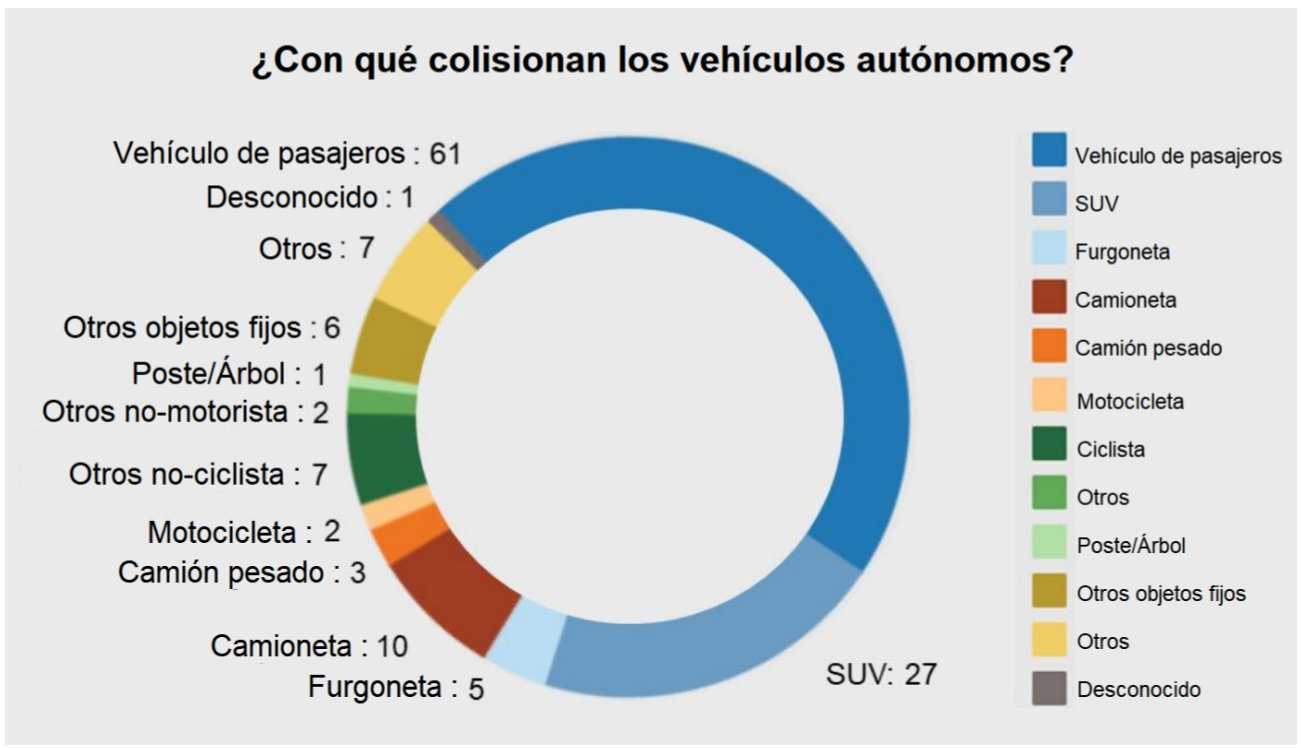
\includegraphics[width=10.5cm]{figures/2.3.png}
  \caption{\label{fig:2.3} Colisiones de vehículos autónomos en niveles 3-5 (original en \textcite{nhtsa22b}.}
\end{figure}

Los principales daños para vehículos de niveles inferiores fueron en la parte frontal del vehículo (frontal, seguido de frontal-izquierdo y frontal-derecho), todo lo contrario que los vehículos de niveles superiores, donde los daños se produjeron especialmente en la parte trasera (trasera, seguido de trasera-izquierda y trasera-derecha).
El conjunto de los resultados permite discernir que en la conducción automatizada existen diferentes modos de conducción y que, por tanto, los problemas que puedan surgir en cada uno de los niveles deben de estudiarse independientemente. Los alcances frontales para los vehículos equipados con \gls{adas}, donde es necesaria la intervención del conductor, sugieren que una confianza excesiva en el sistema, que repercute en una falta de atención y una reacción tardía del conductor ante un evento inesperado (\cite{cunningham}; \cite{yang21}; \cite{mcwilliams}; \cite{hsieh}). Por contra, en los vehículos altamente automatizados los daños traseros se podrían relacionar con frenadas bruscas, que apuntan a un problema de error de percepción, donde se detectan obstáculos que no existen, denominado comúnmente como falsos positivos (\cite{bellosalau}; \cite{buhler}; \cite{zhang22}). Estas dos hipótesis han sido ampliamente estudiadas por la comunidad científica, como se observa en los siguientes apartados, abriendo un abanico de líneas de investigación para cada una con objeto de mejorar la conducción autónoma en todas sus facetas.

\subsection{Conducción parcialmente automatizada}
En los últimos años, la industria del automóvil ha contribuido al desarrollo de distintos dispositivos de protección para mejorar la seguridad en la conducción, desde el cinturón de seguridad hasta los sistemas de ayuda a la conducción. A través de esta tecnología es posible controlar y limitar factores tan importantes como el entorno o el error humano, asistiendo al conductor en la toma de decisiones y recomendándole medidas ante situaciones potencialmente peligrosas (\cite{schoegg}). Estos sistemas cobran especial importancia en los niveles 1 y 2, encargándose del control de bajo nivel, ya sea parcial o totalmente. La presencia de sensores de percepción del entorno como cámaras, radares o láseres, entre otros, permiten que el vehículo ejecute ciertas acciones básicas de forma independiente, pero siempre con la supervisión del conductor. Sin embargo, estos primeros niveles son sensibles a una mala praxis por parte del conductor, ya que se enfrenta a una forma diferente de conducir, donde físicamente podría abandonar alguno de los controles, pero cognitivamente no puede salir el bucle de control. Estudiar su comportamiento es fundamental para el desarrollo y la implementación de sistemas funcionales cuyo fin sea mejorar la seguridad en carretera. 

En este punto, se encuentran estudios sobre la interacción con sistemas de ayuda en conducción parcialmente automatizada que abordan problemas como el rendimiento en la realización de tareas secundarias (\gls{ndrt}), la atención dividida en la monitorización del entorno y la recuperación de la toma de control del vehículo (\cite{naujoks16}; \cite{solismarcos}; \cite{hensch}; \cite{zangi}; \cite{li22a}). La activación de sistemas de ayuda a la conducción reduce la frecuencia de eventos y estímulos para el conductor, incitándole a la realización de tareas distractoras y dando lugar a una monitorización pasiva del entorno (\cite{endsley}). Este hecho compromete la seguridad de la conducción ya que derivaría en una anticipación deficiente ante la aparición de un evento crítico. La falta de atención o las distracciones son elementos a evitar en cualquier tipo de conducción, debido a que suponen un gran porcentaje de las colisiones que se producen en tráfico real como se expone en \textcite{neale}, donde el 78\% de las colisiones y el 65\% de las casi colisiones se debían a esta causa.

No obstante, se encuentran aportaciones interesantes que plantean soluciones constructivas en este asunto. En \textcite{lee19} se observó que el efecto de entablar una conversación disminuye significativamente la fatiga y el aburrimiento del conductor generado por la automatización en el nivel 2 de su vehículo. Numerosos autores se apoyan en analizar el comportamiento visual del conductor para obtener resultados sobre la carga mental que suponen estas situaciones y posibles mejoras en el diseño para favorecer las capacidades del conductor (\cite{forster}; \cite{chen}; \cite{ulahannan}; \cite{goncalves}). Este conocimiento ayuda a la caracterización del conductor, la cual se debe de contemplar dentro de los algoritmos de control del vehículo, facilitando la maniobrabilidad del conductor y evitando problemas derivados de la falta de atención y las distracciones (\cite{ahlstrom}; \cite{cunningham}). Aunque estos dilemas estén más presentes en la conducción parcialmente automatizada, también son aplicables a niveles superiores de automatización donde se requiera la intervención del conductor ante un evento crítico (\cite{jimenez18}; \cite{morales}; \cite{merlhiot}).

\subsection{Conducción altamente automatizada}
La realidad que parece más cercana es la conducción parcialmente automatizada, implementando poco a poco cada uno de los niveles de automatización en la sociedad actual. Sin embargo, existen vertientes que sugieren que el éxito del vehículo autónomo reside en particularizar el entorno por el que circule, eludiendo la problemática que entraña el tráfico mixto (\cite{ma}; \cite{zhang20}). La creación de un carril específico para vehículos altamente automatizados beneficiaría tanto a los usuarios como a los demás vehículos del entorno, eliminando la necesidad de un conductor y estableciendo un transporte tan seguro como el tren o el metro. De esta manera, se promovería la confianza en la tecnología de conducción autónoma y se reduciría la probabilidad de accidentes causados por errores humanos (\cite{nickkar}; \cite{zhang20}; \cite{sohrabi}). Sin embargo, esta solución puede alterar la capacidad de la vía debido al aumento del flujo de tráfico en caso de no tener espacio suficiente para la creación de este carril exclusivo (\cite{ghanipoor}; \cite{santana}).

A pesar de que los vehículos altamente automatizados prometen una mayor seguridad en la carretera al reducir los errores humanos, la convivencia con los vehículos convencionales en el tráfico mixto puede implicar ciertas complicaciones debido a la interacción entre los mismos. Relacionado con ello, los autores \textcite{favaro} y \textcite{petrovic} analizaron una base de datos de accidentes donde estuvieron involucrados vehículos con algún grado de autonomía. Entre los vehículos analizados destacaron los niveles de autonomía 4 y 5, ya que la empresa Waymo reportó la mayor cantidad de informes, debido a su mayor flota y kilometraje recorrido en comparación con otros fabricantes. En ambos estudios se obtuvo que las colisiones traseras con un vehículo convencional fueron el accidente más frecuente, señalando a un posible error humano causado por una conducción demasiado cercana al vehículo delantero o una velocidad insegura. Dinámicamente, los vehículos autónomos se comportan diferente a los convencionales, lo cual puede resultar confuso para un conductor humano cuyo concepto de velocidad y aceleración no es tan suave y gradual. En el estudio de Petrović se sugiere la colocación de una señal en la parte trasera del vehículo que indique que se trata de un vehículo autónomo, con objeto de advertir sobre la posibilidad de que presente acciones imprevistas. Además, destaca la importancia de educar a la población sobre las características de los vehículos autónomos en la circulación del tráfico, lo que aumentaría la conciencia sobre las diferencias en las características dinámicas entre los mismos. En este contexto, es importante tomar medidas para mejorar la seguridad en la carretera y aumentar la conciencia sobre las características de los vehículos autónomos.

La confiabilidad de los conductores en vehículos de alta automatización depende en gran medida del riesgo percibido (\cite{li19}) al igual que de la información proyectada por el vehículo mientras está operando en modo autónomo (\cite{danner}). Sin embargo, esta variable puede verse afectada negativamente por la aparición de falsos alarmas en la detección de obstáculos, generando una disminución de la confianza en el sistema debido a la percepción de un nivel de riesgo superior al real (\cite{drexler}). Debido a esto, es necesario el desarrollo de algoritmos precisos capaces de detectar y caracterizar la mayor variedad de anomalías posibles que puedan ocurrir durante la conducción (\cite{bellosalau}). 

\section{La toma de decisiones en conducción autónoma }
Uno de los procesos más importantes en el desarrollo de un vehículo autónomo es el proceso de la toma de decisiones. Los vehículos procesan la información recopilada por los sensores con objeto de identificar obstáculos y situaciones críticas en la carretera, analizando las posibles opciones para determinar la opción más segura. Este proceso se basa en modelos matemáticos, diseñados para imitar la manera en que los conductores responden a diferentes situaciones del entorno. Para poder entender la complejidad de los algoritmos de toma de decisiones es necesario conocer en detalle la base de los modelos de comportamiento del conductor.

\subsection{Modelos de conducción}
La tarea de conducción se puede dividir en dos movimientos principalmente, longitudinal y lateral. Para caracterizar cada una de estas acciones los primeros autores se refirieron a ellas como seguimiento de vehículo o car-following (\cite{reuschel}; \cite{pipes}) y cambio de carril o lane-changing (\cite{sparmann}; \cite{gipps}). Desde entonces, las técnicas de modelado han dado lugar a múltiples desarrollos interesantes que son referencia en los modelos de conducción (\cite{chandler}; \cite{herman59}; \cite{newell}; \cite{gazis}; \cite{bexelius}; \cite{ahmed96}; \cite{halati}; \cite{toledo03}). Numerosas revisiones, entre ellas \textcite{brackstone}, \textcite{olstam} y \textcite{diaz}, analizan su evolución diferenciando cada una de las vertientes propuestas por los autores. 

Ambas acciones han de analizarse en conjunto ya que, de manera general, la maniobra de cambio de carril tiene su inicio en un ajuste de velocidad respecto al vehículo que le precede. Los criterios en la toma de decisiones durante este proceso han suscitado diversas teorías para predicción del comportamiento del conductor. Una de las más populares es la aceptación de huecos o gap-acceptance, la cual se estudia en las publicaciones de \textcite{herman61}, \textcite{drew} y \textcite{miller}, en diferentes distribuciones. Factores como el tipo de cambio, la velocidad del líder, la distancia hasta al final del carril, la cooperación entre vehículos, los huecos rechazados y el tiempo de espera dieron paso a numerosos estudios en el análisis de su ejecución (\cite{mahmassani}; \cite{gipps}; \cite{madanat}; \cite{cassidy}; \cite{ahmed96}; \cite{yang96}; \cite{halati}; \cite{hidas}; \cite{toledo07}).

\begin{figure}[h]
  \centering
  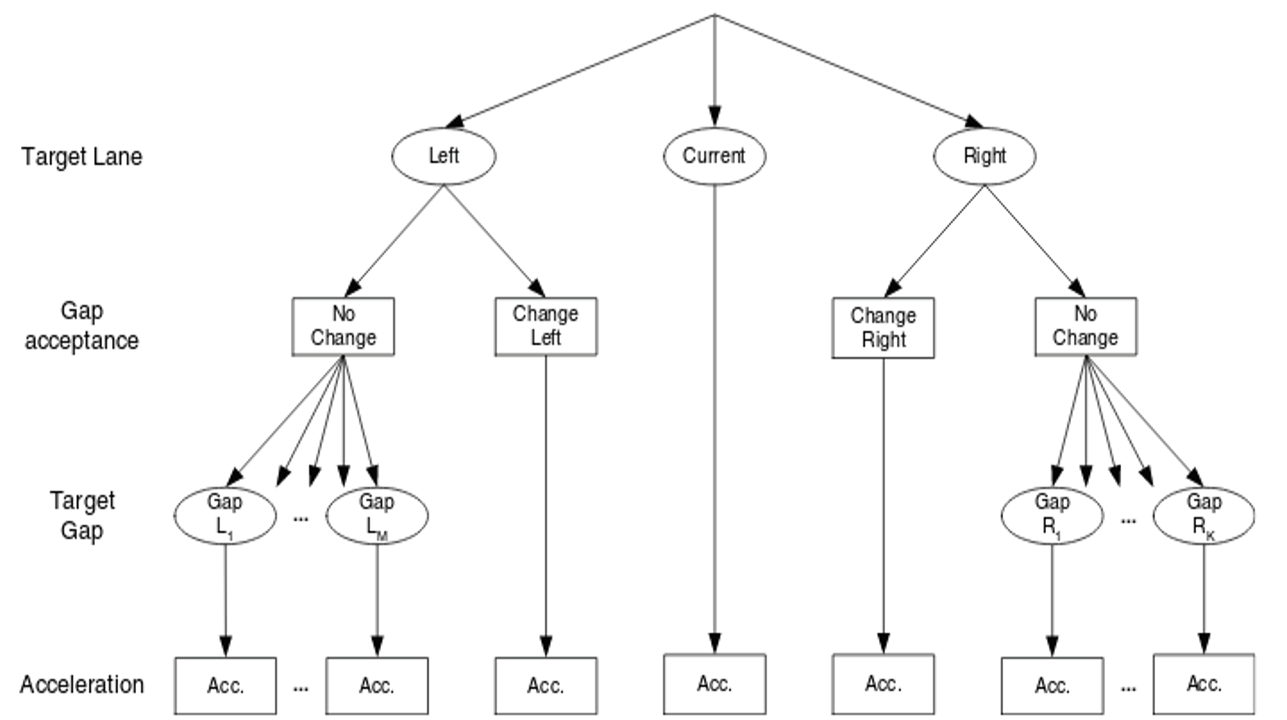
\includegraphics[width=12.5cm]{figures/2.4.png}
  \caption{\label{fig:2.4} Estructura del modelo de comportamiento de los vehículos (\cite{toledo07}).}
\end{figure}

El comportamiento del conductor no adquirió naturalismo hasta la aparición de los modelos psicofísicos (\cite{michaels}; \cite{wiedemann74}) que daría pie a una nueva línea de modelos donde se contemplasen variables cognitivas dando lugar a modelos más predictivos y realistas. Posteriormente el trabajo realizado por \textcite{michon} introdujo los procesos cognitivos en el análisis de las tareas de conducción, dividiendo la tarea en tres niveles jerárquicos, el estratégico, el táctico y el de control, situándose la toma de decisiones en el segundo nivel.

Dado que el entorno y el estado del conductor influyen directamente en las acciones que realiza, se establecieron subdivisiones dentro de los movimientos principales de la conducción llamados regímenes. Ejemplo de ello es la investigación publicada por \textcite{wiedemann92}, donde se presentó un modelo psicofísico de seguimiento de vehículo definido por diferentes regímenes de aceleración (aceleración libre, seguimiento de vehículo, acercamiento y emergencia). En \textcite{sharma19} se identificaron hasta seis regímenes diferentes para completar una trayectoria, definidos como aceleración, aceleración libre, seguimiento, crucero, desaceleración y parada. 

Por otro lado, los modelos de predicción también son clasificados según sus características conceptuales, diferenciando entre modelos deterministas, cuya ventaja principal es que son más fáciles de desarrollar y sus resultados son repetibles, y los modelos estocásticos, que incluyen  procesos aleatorios pudiendo abarcar muestras de gran tamaño y contemplando incertidumbres significativas. En ambos planteamientos se han realizado estudios interesantes, como es el caso de \textcite{vanbrummelen}, donde se desarrolló un modelo probabilístico al estacionamiento de un vehículo aplicado a la conducción autónoma. En predicción probabilística se encuentran diversos trabajos relacionados con el proceso de decisión de Markov, en su forma oculta y parcialmente observable, en el campo de la conducción autónoma (\cite{guan}; \cite{park}; \cite{li21a}). Pero la diversificación de estas metodologías no incluye su división, ya que en estudios muy recientes (\cite{suh}, \cite{luo}) se propusieron modelos predictivos fusionando el enfoque determinista y probabilista para la decisión de cambio de carril en conducción autónoma.

\subsection{El proceso de decisión en algoritmos naturalistas}

En la conducción autónoma, la toma de decisiones es fundamental para asegurar un desplazamiento seguro y eficiente. En el contexto del tráfico mixto, la comunicación entre vehículos autónomos y vehículos conducidos por humanos debe ser lo más análoga posible, evitando situaciones confusas que puedan derivar en malentendidos o accidentes (\cite{jenssen}). Por ello, la capacidad de comprender las intenciones de otros vehículos se convierte en una tarea fundamental para el vehículo autónomo. Aunque esta habilidad sea característica de un conductor real, los algoritmos de percepción y toma de decisiones deben ser capaces de comprender y anticipar las acciones humanas para garantizar una conducción confiable. De igual manera, la respuesta del vehículo autónomo debe ser adecuada y comparable a la que realizaría cualquier conductor en el mismo entorno, con objeto de que los demás vehículos puedan advertir claramente sus intenciones. 

Para lograr una respuesta adecuada del vehículo autónomo, es importante tener en cuenta la caracterización del conductor y el análisis de su comportamiento frente a diversas situaciones, tanto cotidianas como complejas. Sin embargo, la comprensión completa de los factores humanos y los procesos de toma de decisiones durante la conducción debe de ser contemplada desde un enfoque interdisciplinar y colaborativo, incluyendo profesionales del sector de la ingeniería, la psicología y la industria del transporte (\cite{cacciabue}). Los desarrollos de toma de decisiones basados en conducción naturalista abordan este problema mediante la identificación de patrones y reglas de comportamiento de los conductores a través de datos adquiridos de situaciones reales. La información es recogida de los sensores ubicados en el vehículo y el propio conductor, procediendo bien del posicionamiento del vehículo, como son acelerómetros, giróscopos o sistemas de posicionamiento; del entorno exterior, englobando los sistemas radar, los sistemas de detección y medición de distancias por luz, en inglés \gls{lidar} y las cámaras; o de la fisiología del conductor, evaluando su comportamiento visual, actividad cerebral o respuestas físicas. La toma de decisiones naturalista ha sido ampliamente estudiada, siendo su principal foco la caracterización de maniobras en entornos complejos, como son rotondas (\cite{cuenca}; \cite{kong}), cambios de carril (\cite{yang19}; \cite{shawky}; \cite{ali21}) e incorporaciones a una vía principal (\cite{kang}; \cite{gu}). Los estudios naturalistas pueden generar grandes volúmenes de información que permiten extraer patrones concretos de conducción a través de la observación de variables. Analizando estos datos es posible construir modelos que describan de forma estadística la realización de determinadas maniobras durante la conducción (\cite{bender}), extrayendo información del entorno o del propio conductor. 

Por otro lado, también se encuentran repositorios muy completos donde se analizan variables fisiológicas del conductor, como es el movimiento de los ojos y de la cabeza, para perfeccionar la determinación de un cambio de carril (\cite{deng}). En la investigación desarrollada por \textcite{xia}, se hace referencia al mecanismo de atención selectiva del sistema de visión humana para crear un modelo de intención de cambio de carril naturalista. En otros estudios de la misma índole, se analiza la actividad cerebral de los conductores para la modelización de su comportamiento en la realización de rotondas (\cite{monsalve}). Centrado en el vehículo autónomo, los patrones visuales aportan información sobre el estado de desconexión de un conductor durante el uso del piloto automático de un vehículo Tesla (\cite{morando}), elaborando un modelo basado en datos de conducción naturalista a través de diferentes sensores, tanto exteriores como interiores al vehículo. De igual forma, los sistemas de ayuda a la conducción son comúnmente evaluados por sistemas de seguimiento visual (\cite{sanchez}; \cite{azevedo}; \cite{schindler}; \cite{zhou}), los cuales aportan información relevante sobre su diseño y operatividad.

Enfatizando en los sistemas de seguimiento visual, es importante destacar su relación con las intenciones del conductor, ya que ayuda a la generación de reglas de decisión para la mejora de algoritmos de toma de decisiones. El comportamiento ocular de un conductor durante la exploración de una escena, puede ser una herramienta valiosa en el desarrollo de planificaciones previas al proceso de decisión. En \textcite{lappi} se realizó un estudio naturalista enfocado a la estrategia de la mirada del conductor, resumiendo en siete los objetivos mirados más relevantes, los cuales fueron la mirada a la carretera o al infinito, a los instrumentos y espejos retrovisores, a intersecciones, señalizaciones, elementos físicos de la carretera y a la propia escena global. Conocer las variables más importantes para el conductor es una cuestión fundamental en la elaboración del algoritmo de control para un vehículo autónomo cuyo entorno actual es el tráfico mixto. 

\subsection{Factores en el modelado del conductor}
La conducción es un proceso complejo que implica la consideración de múltiples factores, los cuales pueden afectar significativamente en el sistema decisión. La diversidad de variables es tan amplia que, ante un mismo entorno, se pueden tener soluciones totalmente opuestas. Por ello, es importante definir los parámetros que regirán el funcionamiento del modelo y tener en consideración los factores no contemplados con el fin de obtener resultados precisos y confiables.  

Numerosos autores han identificado parámetros importantes en el proceso de modelización (\cite{cacciabue}; \cite{hole}; \cite{saifuzzaman}; \cite{jimenez17}). En este último trabajo, Jiménez se llevó a cabo un análisis detallado de las distintas dimensiones que conforman los factores humanos en la conducción, presentando un mapa donde se muestran los diversos factores que influyen en el estilo de conducción, resumidos en factores humanos, ambientales y vehiculares (Figura \ref{fig:2.5}). 

\begin{figure}[h]
    \centering
    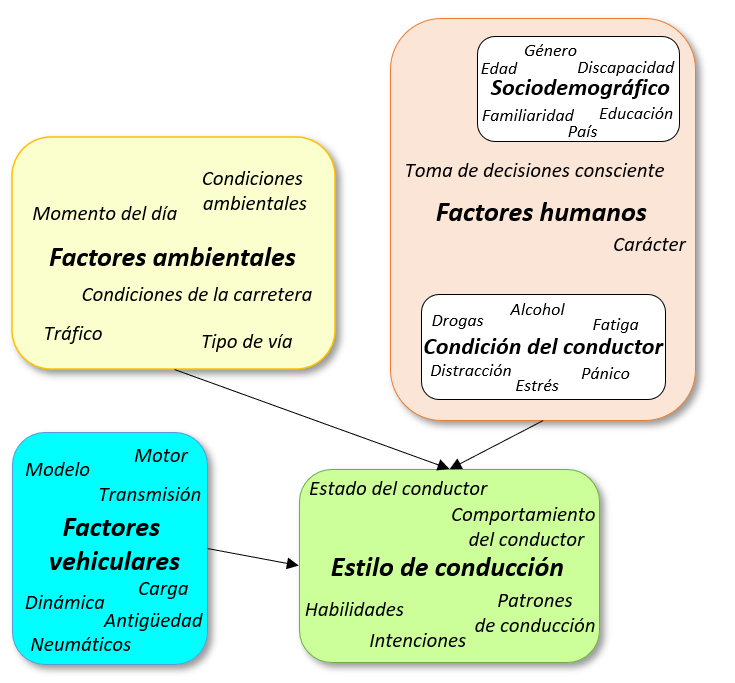
\includegraphics[width=10.5cm]
    {figures/2.5.png}
    \caption{ \label{fig:2.5} Factores relacionados con la conducción humana (original en \cite{jimenez17})}
\end{figure}

Por otro lado, en \textcite{bonsall} se estudian los parámetros relacionados con la seguridad en los modelos de simulación de tráfico, los cuales engloban submodelos de comportamiento relacionados con el seguimiento de vehículo, aceptación de huecos y cambio de carril. Los principales parámetros se resumen en velocidad y avance deseado, tasa de aceleración y deceleración, tiempo de reacción, hueco aceptable, crítico y mínimo en la realización de maniobras de cambio de carril.
Considerando los desarrollos propuestos en esta tesis, en los siguientes apartados se profundizará en los estudios previos relacionados con las variables de aceleración, deceleración, tiempo de reacción y hueco aceptable. La elección de unos valores óptimos y adecuados permitirá una modelización precisa del comportamiento del conductor y, por tanto, contribuirá en una mejora en el diseño de los algoritmos de conducción autónoma.

\subsubsection{2.2.3.1	Niveles de aceleración y deceleración}

La parametrización de un modelo de comportamiento del conductor implica considerar diversos factores, donde la dinámica longitudinal es uno de los más importantes. La capacidad de aceleración y deceleración del vehículo es un factor crucial en la definición de maniobras, sin embargo, su integración en un algoritmo de conducción no es una tarea fácil. En conducción real, estos parámetros son dependientes de las características del vehículo y el entorno que le rodea, como es el estado de la carretera o la suavidad con la que se realiza una maniobra, por lo que para cada situación es necesario contemplar un rango especifico. 

A diferencia de los niveles de deceleración, el estudio de los niveles de aceleración son un tema complejo, debido a su dependencia con la marcha en la que el vehículo se encuentra operando. No obstante, existen estudios que definen rangos de operación para aplicaciones donde es necesario definir unos límites de aceleración y frenado en el diseño de algoritmos de conducción. En \textcite{vanarem} se evaluó el impacto de un sistema de control crucero adaptativo a través de simulación, estableciendo unos valores de aceleraciones máximas confortables de 2 m/s$^2$ y -3 m/s$^2$, en aceleración y deceleración respectivamente. Sin embargo, para el mismo caso de estudio, en \textcite{yi} se consideró que este rango debería ser más estrecho, estando comprendido entre 1 m/s$^2$ a -2.5 m/s$^2$. Por otro lado, \textcite{prestl} estableció un intervalo de 1 m/s$^2$ a -2 m/s$^2$ en concepto de aceleraciones para el desarrollo de un sistema inteligente, con objeto de evitar problemas en el flujo del tráfico en caso de una decisión poco apropiada. 

En el estudio naturalista planteado por \textcite{danaher} se analizó el comportamiento del conductor en las diferentes fases de aceleración entre dos intersecciones, obteniendo valores de aceleración promedio de 0.12g para el primer segundo, 0.26g del segundo hasta el tercero, 0.22g hasta el quinto y 0.17g hasta el séptimo. En materia de desaceleración desde el pico máximo hasta su detención total obtuvo 0.19g desde el primer segundo hasta el sexto y 0.09g del sexto al octavo. La aceleración media en intersecciones señalizadas también fue objeto de investigación en \textcite{almallah} junto al tiempo de reacción y la sobreaceleración, obteniendo valores de 2.8 m/s$^2$ de media para la variable en cuestión.

En la actualización sobre la teoría del flujo de tráfico realizado por \textcite{gartner}, también se aborda el proceso de aceleración, considerando rangos nominales entre 0.6 m/s$^2$ y 0.7 m/s$^2$ para una aceleración confortable a velocidades a partir de 48 km/h. En situaciones donde los conductores circulan con urgencia, se encuentran valores superiores que llegarían a estar alrededor de 1 m/s$^2$. Estudios naturalistas más recientes, obtuvieron resultados similares a los anteriores en la evaluación de diferentes modelos de seguimiento de vehículos (\cite{he}), aunque también respaldan que los valores de aceleración no se ven influenciados por el estilo de conducción a nivel estadístico (\cite{lyu}).

En relación con la deceleración o frenada de un vehículo se encuentran diversos estudios dedicados al análisis y a la caracterización de esta acción. Un ejemplo de ello son las condiciones de frenado que establece la normativa europea (\cite{frenado}), la cual considera que la deceleración media no debe ser inferior a 5.8 m/s$^2$ a una velocidad de 80 km/h con el motor desembragado, ni inferior 5 m/s$^2$ a una velocidad entre el 80\% de la máxima y 160 km/h con el motor embragado. En \textcite{roenitz} se observó que la desaceleración no era lineal a velocidades bajas, entre 20 y 30 km/h, obteniendo valores de 0.25g (aproximadamente 2.452 m/s$^2$) ante un peligro esperado. La Asociación Estadounidense de Oficiales de Carreteras Estatales y Transportes (\gls{aashto}) sugieren deceleraciones del orden de 2 m/s$^2$ a 2.6 m/s$^2$ en el Libro Verde sobre diseño geométrico de carreteras y calles (\cite{AASHTO}).

Al igual que con la aceleración, en \textcite{gartner} se estudia el comportamiento de la deceleración, analizando los casos de frenado en bucle abierto y bucle cerrado. En el caso que un conductor se encontrase con un obstáculo inesperado y realizase una maniobra de frenado ejerciendo la máxima fuerza posible sobre el pedal, estaría en bucle abierto. Para este caso y teniendo un vehículo de gran tamaño sin sistema de frenos antibloqueo (\gls{abs}),se obtuvieron aceleraciones de 0.7g en una parada estacionaria, siendo los valores pico de 0.9g. En las mismas condiciones, pero con asfalto mojado, las aceleraciones alcanzaron valores de 0.4g. En el caso de bucle cerrado, el cual correspondería a una frenada controlada donde el conductor busca una deceleración confortable, los valores oscilaron entre 0.46g y 0.70g, siendo de 0.55g de media para un obstáculo inesperado y 0.45g para un obstáculo esperado. El valor de una deceleración cómoda se considera 0.3g, sin embargo, los autores estiman que debería de estar alrededor de 0.35g para una situación más realista. 

La caracterización de la deceleración ha sido abordada con mayor profundidad en los desarrollos dedicados al análisis de colisiones por alcance. En el trabajo realizado por \textcite{burgett98} para el desarrollo de un algoritmo de aviso de colisión, se asumió una deceleración constante máxima de 0.75g, teniendo en cuenta una situación en la que vehículo predecesor se detenga en condiciones óptimas. Posteriormente el mismo autor (\cite{burgett01}) establecería tres niveles de sensibilidad a este valor, correspondiendo a una sensibilidad baja 0.6g, media a 0.5g y alta 0.4g. De la misma manera, en \textcite{wilson} se utilizó un valor de deceleración máxima conservadora de 0.75g para la evaluación de un accidente por alcance, todo lo contrario que en \textcite{weaver11}, donde los valores típicos de aceleración y deceleración para maniobras realizadas en tráfico urbano, no superaron los 0.35g para ambas aceleraciones.

El estudio presentado por \textcite{das} proporciona una visión completa del ajuste de parámetros de desaceleración para un cambio de carril obligatorio en función de las condiciones climáticas, diferenciando ente despejado, lluvia ligera, lluvia pesada, nieve ligera, fuertes nevadas, niebla distante y niebla densa. Los datos obtenidos para el propio vehículo contemplan un amplio espectro de valores desde 26.36 ft/s$^2$ de máximo para las situaciones en las que el conductor se enfrenta a una niebla densa, hasta 5.74 ft/s$^2$ de máximo en los casos de lluvia pesada. 

En el contexto de la prevención de colisiones frontales, se han desarrollado diversos estudios en simuladores de conducción para analizar el comportamiento del conductor. En algunos estudios, se registraron valores de desaceleración comprendidos entre 5 m/s$^2$ y 8 m/s$^2$ (\cite{ho}; \cite{bella}). Estudios más actuales apoyan estos rangos respaldando que un umbral de desaceleración de 7.5 m/s$^2$ podría tener un efecto en la mejora de la prevención de colisiones frontales y el tiempo de colisión (\cite{hang}).

En el campo de la conducción autónoma, \textcite{jeong} estudian la optimización de maniobras mediante un algoritmo de control con tres rangos de aceleración, confort (-2 m/s$^2$ a 2 m/s$^2$), deceleración grande (-2 m/s$^2$ a -4 m/s$^2$) y frenada severa (entorno a 8 m/s$^2$). En \textcite{saito} se propuso un sistema de asistencia para controlar la desaceleración del vehículo, cuyo valor frente a una frenada de emergencia fue de 6 m/s$^2$ en promedio. \textcite{naujoks18} analiza diferentes aspectos de la conducción parcialmente automatizada mediante diferentes niveles de automatización en un simulador de conducción, siendo su parámetro de desaceleración igual a 4 m/s$^2$. 

Por último, en \textcite{wang} se hallaron unos umbrales de 0.85 m/s$^2$ y 1.76 m/s$^2$ para la desaceleración mínima en la maniobra de cambio de carril utilizando un modelo de decisión en situaciones de conducción real. El estudio de estos valores es una parte fundamental en la definición de limites seguros de aceleración y desaceleración en los algoritmos de conducción centrados en vehículos autónomos con el fin de mejorar la seguridad en la carretera.

\subsubsection{2.2.3.2	Tiempo de reacción}

Una de las principales diferencias en el comportamiento durante la conducción entre conductores humanos y máquinas es el tiempo de reacción, los puntos de reacción y el tiempo de adelantamiento (\cite{wagner}). Entre ellas, el tiempo de reacción, es una variable importante en la modelización de ciertas maniobras, debido a que la percepción humana de un estímulo no implica una respuesta automática por parte del conductor. Si bien es cierto que el tiempo de reacción se encuentra influenciado por diversos factores como la edad, la fatiga, el nivel de atención o el consumo de sustancias, se encuentran extensas revisiones que determinan rangos de operación enfocados a un mayor conocimiento para su implementación de modelos y simuladores de conducción (\cite{greenshields}; \cite{sens}; \cite{olson}; \cite{green}; \cite{gartner}).

El tiempo de reacción se compone de dos elementos, tiempo de percepción, donde el conductor obtiene la información sobre el estímulo y decide la respuesta que necesita ante esa reacción, y tiempo de maniobra, que implica la ejecución de la maniobra que se va a realizar y el tiempo que tarda en completarla (\cite{mclaughlin}). \textcite{hooper} dividieron el tiempo en tres fases, percepción, decisión y respuesta, diferenciando dentro de percepción los procesos de latencia, movimiento ocular o sacada, fijación y reconocimiento. Además, propusieron una clasificación por percentiles siendo de 3.5 segundos el valor correspondiente al total del tiempo de reacción para una frenada en un 90\% de la población. 

El diseño de carreteras es una de las aplicaciones más comunes en las que interviene el tiempo de reacción. La planificación de las intersecciones, el ancho de la carretera, el diseño de las señales de tráfico, son, entre otros, factores que dependientes de este tiempo, dado que una buena ingeniería en la infraestructura garantiza la seguridad de los conductores y los demás usuarios de la vía. En España, por ejemplo, el Ministerio de Obras Públicas y Urbanismo ha establecido un tiempo de reacción de 2 segundos (\cite{mopu}) para los diseños de las carreteras. En algunos países como Estados Unidos, se ha adoptado un valor de 2.5 segundos como criterio de diseño para la infraestructura vial (\cite{AASHTO}). Otros protocolos de diseño de carreteras, como el Indian Road Congress (\cite{irc}), también se adhieren al estándar establecido por la Asociación Estadounidense de Funcionarios de Carreteras y Transportes (\gls{aashto}).

En otro punto, el Código de la Circulación del Reino Unido (The Official Highway Code) emplea un valor de 2 segundos para para determinar un margen de seguridad durante la conducción en la realización de maniobras como los adelantamientos (\cite{department}). Por otro lado, el Consejo Nacional de Seguridad americano (\gls{nsc}) recomienda una separación mínima de 3 segundos entre los vehículos que circulen por el mismo carril. No obstante, los tiempos de reacción de los conductores humanos varían en un rango reducido, desde 0.9 a 1.2 segundos (\cite{johansson}) o de 0.5 a 2 segundos (\cite{aparicio}; \cite{orosz}). 

En el ámbito de la conducción autónoma, el tiempo de reacción es uno de los factores más presentes en relación con el factor humano, considerado desde el diseño de sistemas de seguridad y tecnologías de asistencia al conductor, hasta la operatividad de los sistemas de decisiones y toma de control. En el estudio de \textcite{jimenez18}, se evaluaron dos métodos para comprobar si el conductor estaba listo para retomar la conducción en un sistema de conducción autónoma nivel 4, los cuales involucraron la lectura de una palabra o la realización de un cálculo aritmético evaluando el tiempo de respuesta del conductor. \textcite{naujoks18} analizaron el tiempo de reacción y la fatiga en diferentes niveles de conducción ante la realización de una tarea secundaria, obteniendo valores mínimos de 2.02 segundos para una colisión en conducción parcialmente automatizada. El tiempo de reacción también fue estudiado en \textcite{wong}, donde analizaron su variabilidad ante alertas asertivas en un simulador para conducción semiautónoma.

El contexto del tráfico mixto es fundamental tener un conocimiento preciso sobre esta variable, dada la imprevisibilidad del entorno. El flujo de tráfico en un ambiente mixto de vehículos conectados inteligentes es estudiado en \textcite{chang}, donde utiliza valores de tiempos de reacción entre 1.5 y 2 segundo para los vehículos de un modelo de simulación. Aplicado al mismo contexto, \textcite{fu} realiza ensayos en conducción real para la modelización de la situación donde otro vehículo se intercala en el carril del vehículo autónomo, denominada también maniobra de cut-in.

Finalmente, se observa que los sistemas de asistencia al conductor también dependen significativamente de esta variable, especialmente los sistemas de control adaptativo de la velocidad. Algunos sistemas permiten que el conductor introduzca el tiempo que desea que se mantenga de separación con respecto al vehículo precedente, lo que se traduce en una distancia variable en función de la velocidad (\textcite{prestl}). En el mismo caso, \textcite{pomerleau} basa su investigación en comunicación entre vehículos para detectar situaciones de riesgo, recomendando usar valores superiores a 1.5 segundos.

\subsubsection{2.2.3.3	Hueco aceptable}

En la modelización de las maniobras de desplazamiento lateral, como las incorporaciones o el cambio de carril, la aceptación de hueco es un parámetro determinante para la toma de decisiones. Un modelo clave en esta materia es el modelo  \textcite{gipps}, que establece que los conductores ajustan su velocidad y distancia respecto al vehículo delantero para mantener un hueco aceptable que les permita reaccionar ante imprevistos. Diversos estudios de simulación sobre la aceptabilidad de huecos diferencian entre el hueco hasta el vehículo delantero y hasta el vehículo trasero (\cite{kang}; \cite{sharma20}; \cite{pakzadnia}), influyendo ambos en la decisión de aceptación o rechazo de la maniobra.

La determinación del hueco aceptable entre vehículos puede verse influenciada por la complejidad del escenario y el estado del conductor. Estudios como \textcite{paschalidis}, donde utilizaron sensores fisiológicos y modelos de conducción, evidenciaron que un nivel alto de estrés puede tener un impacto significativo en la toma de decisiones. El hueco aceptable es el más generalista en literatura, sin embargo, algunos estudios particularizan este parámetro en función del contexto (\cite{bonsall}; \cite{sanik}; \cite{virdi}; \cite{yang19}), creando modelos más específicos. Además del hueco aceptable, también se han definido otros conceptos como el hueco mínimo de seguridad, relacionado con la distancia mínima con el vehículo delantero, y el hueco crítico y el intermedio, que están relacionados con el cambio de carril y se refieren a situaciones en las que el vehículo trasero puede colisionar si no se toman las medidas adecuadas.

Aplicado a la industria de los vehículos autónomos, algunos autores se apoyan en dicho parámetro para el desarrollo de algoritmos que faciliten la maniobra de incorporación (\cite{scarinci}), ya que a través de esta métrica son capaces de ajustar su velocidad y distancia de manera más precisa. Un ejemplo de ello es el estudio presentado por \textcite{karbalaieali}, en el que se desarrolla un algoritmo adaptativo para guiar a los vehículos que se encuentran en un pelotón al realizar una incorporación a una vía principal, planteando tres puntos de fusión, delante de la formación, detrás y en medio del mismo.

Relacionado con este último punto, los entornos conectados favorecen al desarrollo de formaciones de vehículos en pelotón, optimizando el control del hueco aceptable gracias al intercambio de información en tiempo real. Según \textcite{ali18}, la conectividad de un entorno tiene un efecto significativo en la maniobra de cambio de carril, como muestran en su trabajo donde observaron que los vehículos mantienen distancias más grandes, o más seguras, con el vehículo delantero que en conducción normal. El tamaño de los huecos entre pelotones de vehículos conectados también es objeto de interés en algunas investigaciones (\cite{aramrattana}), encontrándose una mayor satisfacción por parte de los conductores en los huecos mayores de 30 de metros, observándose una ejecución más suave de las maniobras y una menor cantidad de colisiones.

\section{Sensores y variables en el modelado}

La obtención de datos reales es fundamental para desarrollar un modelado preciso y fiable en cualquier sistema de carácter naturalista. En conducción autónoma es imprescindible el uso de sensores para captar la información del entorno exterior, lo que permitirá al vehículo adoptar un comportamiento adecuado en función del contexto en el que se encuentre.

\subsection{Caracterización del vehículo y del entorno}

El uso de sistemas de percepción de vehículos es fundamental para la correcta caracterización del entorno en el que se mueve el vehículo y para la comprensión de las maniobras que se realicen en él. Tanto los fabricantes como la comunidad científica han trabajado ampliamente con diversas tecnologías para mejorar el control de vehículos autónomos y su retroalimentación, para tomar decisiones en función de otros vehículos y así mejorar su capacidad de control y conducción. 

Entre los sistemas más comunes de detección del entorno se encuentran la visión artificial, el \gls{lidar} y el radar, que adquieren fundamentalmente mediciones de distancia entre los vehículos para calcular velocidades y mapas. Por un lado, los sistemas basados en radar proporcionan mediciones directas del efecto Doppler, lo que permite detectar la velocidad relativa de otros vehículos. En otro, los sistemas de visión por computadora también se utilizan como parte de los sistemas de control de crucero adaptativo comerciales (\gls{acc}) y tienen un rango de detección más largo que los sistemas de radar. De manera similar, los sistemas \gls{lidar} emiten un haz de luz enfocado que en su retorno aporta información sobre distancia entre un objeto y el origen del sistema. Entre ellos, los sistemas de visión son el método más extendido en el desarrollo de sistemas de asistencia al conductor, como son el sistema de advertencia de salida de carril (\gls{ldw}), control de crucero adaptativo y sistemas de mantenimiento de carril (\gls{lks}). No obstante, cada vez más se encuentran vehículos comerciales equipados con radar y \gls{lidar}, reforzando la robustez de estos sistemas mediante la redundancia de sensores y la adición de nuevas características, como la frenada de emergencia automática (\gls{aeb}), la alerta de colisión frontal (\gls{fca}), detector de punto ciego (\gls{bsd}) y el asistente de cambio de carril (\gls{lca}).

Los sistemas de posicionamiento han sido ampliamente utilizados en los \gls{adas} para mejorar la precisión de la información de posición y velocidad. Existen varios sistemas de navegación por satélite, pero los más conocidos son el Sistema de Posicionamiento Global (\gls{gps}), el Sistema Global de Navegación por Satélite \gls{glonass}, el Sistema de Navegación por Satélite europeo Galileo y el Sistema de Posicionamiento de China (BeiDou). Cada sistema consta de una constelación de satélites que transmiten señales a los receptores en la Tierra para proporcionar información precisa sobre la ubicación y el tiempo. 

La transmisión de información sobre la posición y la velocidad de los vehículos en tiempo real se logra a través de los sistemas de comunicación inalámbrica, también conocidos como \gls{v2x} y más concretamente como \gls{v2v} cuando se transmite entre vehículos y \gls{v2i} cuando se trata de una infraestructura de la carretera. Esta información es utilizada comúnmente para detectar posibles conflictos y alertar a los conductores, así como para optimizar el tráfico y mejorar la gestión del flujo de vehículos. La conectividad en los vehículos es una de las funciones clave de los sistemas de transporte inteligentes (\gls{its}), desempeñando un papel importante en el desarrollo de vehículos autónomos y la movilidad conectada en el futuro.

\subsection{Comportamiento del conductor a través de la información visual}

La adquisición de variables fisiológicas del conductor, tales como la frecuencia cardíaca, la sudoración y la actividad cerebral, son herramientas valiosas para el estudio de la percepción y la toma de decisiones durante la conducción. Entre ellas, el comportamiento ocular es una de las más importantes, ya que el conductor evaluará el entorno en base a la información visual percibida. A su vez, las variables oculares aportan información sobre el estado del mismo, pudiendo identificar situaciones potencialmente peligrosas a través de patrones visuales, como la fatiga, la distracción, la carga mental y la somnolencia. 

La pupila es la principal fuente de la cual derivan las demás variables que se pueden obtener de un sistema de seguimiento visual, como la posición, la dirección de la mirada y el movimiento de los ojos. Los principales movimientos se resumen en sacadas y fijaciones, siendo las sacadas movimientos rápidos que realizan los ojos al cambiar de un punto de interés a otro, y las fijaciones el tiempo entre sacadas. Para la evaluación de un área de interés se suelen utilizar diferentes métricas entorno a estas variables, como la duración y número total de fijaciones, el tiempo transcurrido hasta la primera fijación, la densidad de las mismas, mapas de calor, el diámetro de la pupila, las rutas o patrones visuales, y parpadeos. La interpretación de dichos datos está sujeta a los diversos estudios presentes en literatura, los cuales están enfocados en diferentes situaciones y estímulos cognitivos.

En los sistemas de seguimiento visual se basan principalmente en una fuente infrarroja que facilita la detección de la pupila a través de una cámara de alta velocidad, cuyo soporte puede ser desde sistemas portátiles en forma de gafas hasta elementos fijos que además adquieren información sobre la cabeza del conductor. No obstante, existen otros métodos para la determinación de los movimientos oculares, como es el \gls{eog}, donde se obtiene la diferencia de potencial eléctrica entre dos puntos cercanos al ojo. Este método está ampliamente utilizado en estudios relacionados con parpadeos y movimientos hacia la periferia ocular, al igual que en investigaciones de los sueños, ya que permite su utilización con los ojos cerrados. Las técnicas de detección de la pupila se resumen en pupila brillante y oscura, diferenciándose en la localización de la fuente de iluminación respecto a los ojos.

La tecnología autónoma y los sistemas de asistencia al conductor utilizan las técnicas de seguimiento visual para mejorar la seguridad en la carretera y la experiencia de los conductores. El desarrollo de aplicaciones para detectar la atención o la fatiga permite prevenir situaciones peligrosas relacionadas con el error humano, alertando al conductor para que se tome un descanso o interviniendo no respondiese. Aplicado a los altos niveles de automatización, donde los conductores pasan largos periodos de tiempo sin controlar activamente el vehículo, el comportamiento visual puede ser una herramienta valiosa para determinar objetivamente si el conductor está preparado para recibir el control del vehículo. 

La combinación de la información visual del conductor con las condiciones del entorno exterior permite obtener una comprensión más completa del entorno y una mejora en la anticipación de eventos potencialmente peligrosos. Dicha combinación no se encuentra muy extendida en los estudios de conducción autónoma, destacando la importancia y la novedad de esta Tesis. La incorporación de estas fuentes de información en los sistemas de asistencia al conductor y en los vehículos autónomos puede tener un impacto significativo en la conciencia situacional y, por ende, en la seguridad y confiabilidad de la operación del vehículo. 
